\documentclass{article}
% Semiconductor Process Flow Template

\usepackage[margin=1cm, top=1.5cm, bottom=1.2cm]{geometry}
\usepackage{fancyhdr}
\usepackage{lastpage}
\usepackage{tabularray}
\UseTblrLibrary{booktabs}
\usepackage{xcolor}
\usepackage{helvet}
\usepackage{siunitx}
\usepackage{amsmath}

\renewcommand{\familydefault}{\sfdefault}

% Custom metadata commands with default values
\newcommand{\processflowtitle}{Semiconductor Fabrication Process}
\newcommand{\revision}{Rev 0.0}
\newcommand{\contactemail}{email@example.com}
\newcommand{\contactname}{Name}
\newcommand{\contactphone}{Phone}
\newcommand{\labmanagergroup}{Group}
\newcommand{\batchname}{Batch}
\newcommand{\datecreation}{YYYY-MM-DD}
\newcommand{\daterevision}{YYYY-MM-DD}

% Footer setup
\pagestyle{fancy}
\fancyhf{}
\renewcommand{\headrulewidth}{0pt}
\fancyfoot[L]{\footnotesize Not confidential}
\fancyfoot[C]{\footnotesize File name: \processflowtitle}
\fancyfoot[R]{\footnotesize Page \thepage\ of \pageref{LastPage}}
\renewcommand{\footrulewidth}{0.4pt}

% Title block command using tabularray
\newcommand{\titleblock}{%
    \centering
    \large
    \begin{tblr}{
        width = \textwidth,
        colspec = {X[1.5,l] X[5,l] X[1.5,l] X[5,l]},
        row{1} = {font=\bfseries},
        row{2} = {abovesep=3pt, belowsep=3pt},
        row{3} = {abovesep=3pt, belowsep=3pt},
        cell{1}{1,3} = {font=\bfseries},
        hlines = {0.5pt, white}, % Hidden lines for alignment
        vlines = {0.5pt, white}, % Hidden lines for alignment
        rowsep = 4pt,
        colsep = 8pt,
    }
        Process flow title: & \processflowtitle & Revision: & \revision \\
        Contact email: & \contactemail & Contact name: & \contactname \\
        Contact phone: & \contactphone &  &  \\
        LabManager group: & \labmanagergroup & Batch name: & \batchname \\
        Date of creation: & \datecreation & Date of revision: & \daterevision \\
    \end{tblr}
    \vspace{1em}
    \hrule height 1pt
    \vspace{2em}
}

% Override default metadata
\renewcommand{\processflowtitle}{Minimal MOS Capacitor Process}
\renewcommand{\revision}{Rev 0.1}
\renewcommand{\contactemail}{jephin@dtu.dk}
\renewcommand{\contactname}{Jeppe Hinrichs}
\renewcommand{\contactphone}{Not applicable}
\renewcommand{\labmanagergroup}{DkCCC}
\renewcommand{\batchname}{TBD}
\renewcommand{\datecreation}{2025-08-15}
\renewcommand{\daterevision}{2025-08-15}

\begin{document}

% First page with title block
\titleblock

% ==== DOCUMENT CONTENT ====
\section*{Process Overview}

Bare-minimum fabrication flow for MOS capacitor structure. \\

\subsection*{Key Specifications}
\begin{itemize}
    \item Gate oxide: \qty{35}{\nano\meter} thermal SiO\textsubscript{2}
    \item Gate electrode: \qty{400}{\nano\meter} n+ polysilicon
    \item Backside contact: \qty{400}{\nano\meter} aluminum
\end{itemize}

\subsection*{Critical Safety}
\begin{itemize}
    \item \textbf{HF handling:} Double nitrile gloves + face shield
    \item \textbf{Furnace:} Thermal gloves for >\qty{800}{\degreeCelsius} operations
\end{itemize}

% === MATERIAL SPECIFICATIONS ===
\section{Starting Material}
\begin{tblr}{
    colspec = {lcc},
    row{1} = {font=\bfseries},
    row{2} = {abovesep=3pt,belowsep=3pt}
}
\toprule
Substrate & Specification & Qty \\
\midrule
Silicon & p-type <100>, 6", 1-10 \Omega\cdot cm & 5 \\
\bottomrule
\end{tblr}

% === LAYER SPECIFICATIONS ===
\section{Critical Layers}
\begin{tblr}{
    colspec = {lcc},
    row{1} = {font=\bfseries},
    row{2-4} = {abovesep=3pt,belowsep=3pt}
}
\toprule
Layer & Material & Thickness \\
\midrule
Gate oxide & Thermal SiO\textsubscript{2} & \qty{35}{\nano\meter} \\
Gate electrode & n+ Poly-Si & \qty{400}{\nano\meter} \\
Back contact & Al & \qty{400}{\nano\meter} \\
\bottomrule
\end{tblr}

% === PROCESS FLOW ===
\section{Core Process Flow}
\begin{tblr}{
    colspec = {cX[3]lX[2]},
    row{1} = {font=\bfseries},
    row{2-5} = {abovesep=3pt,belowsep=3pt}
}
\toprule
Step & Process & Equipment & Key Parameters \\
\midrule
1.1 & RCA clean & Wet bench & SC1+SC2 @ \qty{75}{\degreeCelsius} \\
2.1 & SiO\textsubscript{2} growth & Furnace & \qty{1000}{\degreeCelsius}, 40min \\
3.1 & Poly-Si deposition & LPCVD & \qty{620}{\degreeCelsius}, 2hr \\
4.1 & Gate patterning & Aligner + Etch & Mask: capacitor \\
5.1 & Back Al deposition & E-beam & \qty{400}{\nano\meter} \\
5.2 & Contact anneal & RTP & \qty{450}{\degreeCelsius}, \qty{30}{\minute} \\
\bottomrule
\end{tblr}

% === TROUBLESHOOTING ===
\section{Critical Checks}
\begin{tblr}{
    colspec = {lX[3]},
    row{1} = {font=\bfseries},
    row{2-4} = {abovesep=3pt,belowsep=3pt}
}
\toprule
Step & QC Verification \\
\midrule
2.1 & Oxide thickness: \qty{35}{\nano\meter} ± \qty{1}{\nano\meter} \\
4.1 & Gate CD: ± \qty{0.5}{\micro\meter} \\
5.2 & Contact R < $1~\Omega / \square$ \\
\bottomrule
\end{tblr}

% === FIGURES ===
\section{Required Figures}
\begin{tblr}{
    colspec = {ccX[3]},
    row{1} = {font=\bfseries},
    row{2-3} = {abovesep=3pt,belowsep=3pt}
}
\toprule
ID & Step & Description \\
\midrule
1 & 2.1 &
\begin{minipage}{\linewidth}
    \centering
    {\resizebox{\linewidth}{!}{\resizebox{\linewidth}{!}{%
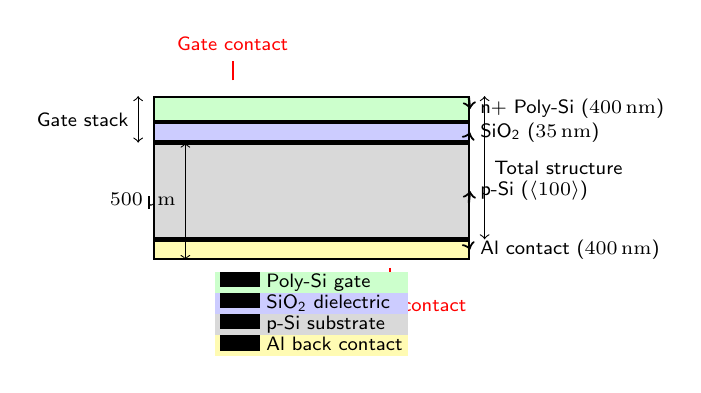
\begin{tikzpicture}[
    layer/.style={draw, thick, minimum width=4cm, minimum height=#1},
    label/.style={midway, align=center, font=\scriptsize}
]

% Heights
\def\subH{1.2}   % Substrate height
\def\oxH{0.15}   % Oxide height
\def\polyH{0.3}  % Poly height
\def\metalH{0.15}% Metal height

% --- Draw layers ---
\node[layer=\subH cm, fill=gray!30] (sub) at (0,0) {};
\node[layer=\metalH cm, fill=yellow!30, anchor=north] (metal) at (sub.south) {};
\node[layer=\oxH cm, fill=blue!20, anchor=south] (ox) at (sub.north) {};
\node[layer=\polyH cm, fill=green!20, anchor=south] (gate) at (ox.north) {};

% --- External labels (staggered arrows) ---
\draw[->, thick] ([xshift=2cm,yshift=0.15cm]gate.center) -- (gate.east)
    node[right, font=\scriptsize] {n+ Poly-Si (\qty{400}{\nano\meter})};

\draw[->, thick] ([xshift=2cm,yshift=-0.05cm]ox.center) -- (ox.east)
    node[right, font=\scriptsize] {SiO\textsubscript{2} (\qty{35}{\nano\meter})};

\draw[->, thick] ([xshift=2cm,yshift=-0.15cm]sub.center) -- (sub.east)
    node[right, font=\scriptsize] {p-Si ($\langle 100 \rangle$)};

\draw[->, thick] ([xshift=2cm,yshift=0.05cm]metal.center) -- (metal.east)
    node[right, font=\scriptsize] {Al contact (\qty{400}{\nano\meter})};

% --- Dimensions ---
% Gate stack
\draw[<->] ([xshift=-2.2cm]gate.north) -- ([xshift=-2.2cm]ox.south) 
    node[label, left] {Gate stack};

% Total structure
\draw[<->] ([xshift=2.2cm]sub.south) -- ([xshift=2.2cm]gate.north) 
    node[label, right] {Total structure};

% Substrate thickness
\draw[<->] ([xshift=-1.6cm]metal.south) -- ([xshift=-1.6cm]sub.north)
    node[label, left] {\qty{500}{\micro\meter}};

% --- Contact points ---
\draw[thick, red] (gate.north) ++(-1,0.2) -- ++(0,0.25) 
    node[above, font=\scriptsize] {Gate contact};
\draw[thick, red] (metal.south) ++(1,-0.1) -- ++(0,-0.25) 
    node[below, font=\scriptsize] {Substrate contact};

% --- Legend ---
\node[anchor=north] at (0, -0.9) {%
    \scriptsize
    \setlength{\tabcolsep}{2pt}%
    \renewcommand{\arraystretch}{0.8}%
    \begin{tabular}{@{}l@{}}
        \cellcolor{green!20}{\rule{5mm}{2mm}} Poly-Si gate \\
        \cellcolor{blue!20}{\rule{5mm}{2mm}} SiO\textsubscript{2} dielectric \\
        \cellcolor{gray!30}{\rule{5mm}{2mm}} p-Si substrate \\
        \cellcolor{yellow!30}{\rule{5mm}{2mm}} Al back contact
    \end{tabular}%
};

\end{tikzpicture}%
}
}}\\[2pt]
    Cross-section
\end{minipage} \\
2 & 5.2 & \begin{minipage}{\linewidth}
    \centering
    %{\resizebox{\linewidth}{!}{\includesvg{moscap_mwe_td.svg}}}\\[2pt]
    Process flow
\end{minipage} \\
\bottomrule
\end{tblr}

\end{document}